\documentclass[t,10pt]{beamer}
\usetheme[official=true, conference=\mbox{N. Vianello
  @ JET 01 June 2012},pagelogo=false]{Rfx}
\usepackage[english]{babel}
\usepackage{listings,amsmath,multimedia}
\usepackage{tangocolors}
\usepackage{rfxcolor}
\usepackage{pgf}
\usepackage{tikz}
%\usepackage[bibstyle=numeric-comp,citestyle=authoryear-comp,labelyear=true,maxnames=1]{biblatex}
%\bibliography{biblio}
%\renewcommand*{\bibfont}{\footnotesize}
\mode<presentation>
\graphicspath{{pdf_box/}}
\renewcommand\Re{\operatorname{Re}}
\renewcommand\Im{\operatorname{Im}}

% for adding foot note with reference
\makeatletter
% add a macro that saves its argument
\newcommand{\footlineextra}[1]{\gdef\insertfootlineextra{#1}}
\newbox\footlineextrabox

% add a beamer template that sets the saved argument in a box.
% The * means that the beamer font and color "footline extra" are automatically added. 
\defbeamertemplate*{footline extra}{default}{
    \begin{beamercolorbox}[ht=2.25ex,dp=1ex,leftskip=\Gm@lmargin]{footline extra}
    \insertfootlineextra
    %\par\vspace{2.5pt}
    \end{beamercolorbox}
}

\addtobeamertemplate{footline}{%
    % set the box with the extra footline material but make it add no vertical space
    \setbox\footlineextrabox=\vbox{\usebeamertemplate*{footline extra}}
    \vskip -\ht\footlineextrabox
    \vskip -\dp\footlineextrabox
    \box\footlineextrabox%
}
{}

% patch \begin{frame} to reset the footline extra material
\let\beamer@original@frame=\frame
\def\frame{\gdef\insertfootlineextra{}\beamer@original@frame}
\footlineextra{}
\makeatother

\setbeamercolor{footline extra}{fg=structure.fg}% for instance

\title{Research \& Coordination  \\
Activity}
\author{N. Vianello }
\date{01 June 2012}

\begin{document}

\begin{titleframe}
\end{titleframe}

\begin{frame}{Personal research interest}
\begin{itemize}
{\large\item Actively involved in fusion plasma science since the
M.Sci. thesis in 1999
\item Personal research interests can be summarized in four main
  macro-areas
\begin{description}
\item[(A)] \textcolor{taorange}{Flows \& Turbulence induced transport in magnetized plasmas}
\item[(B)]\textcolor{ta3chameleon}{Emerging of electromagnetic structures}
\item[(C)] \textcolor{tascarletred}{3D physics and helical plasmas}
\item[(D)] \textcolor{ta3skyblue}{Statistical characterization of
    electromagnetic fluctuations}
\end{description}
}\end{itemize}
\end{frame}

\begin{frame}{Flows \& Turbulence induced transport}


%% per aggiungere la lettera colorata con l'argomento in alto a sx'
\begin{tikzpicture}[remember picture, overlay]
\node [shift={(-0.779 cm,-0.4cm)}]  at (current page.north east)
   {\tikz[baseline=(t1.base)]{\node[fill=taorange](t1){%
{\Large A}};}
    };
\end{tikzpicture}
%%
\begin{itemize}
\item The principal results may be summarized as follows:
\begin{columns}
\onslide<2->{\begin{column}{0.48\textwidth}
{\small \begin{block}{}
(i) Role of electrostatic Reynolds stress in momentum generation in
RFPs, including first measurements of non-linear momentum flux
$\langle \tilde{v}_{\perp}\tilde{v}_r\tilde{n}\rangle$
\end{block}}
\begin{center}
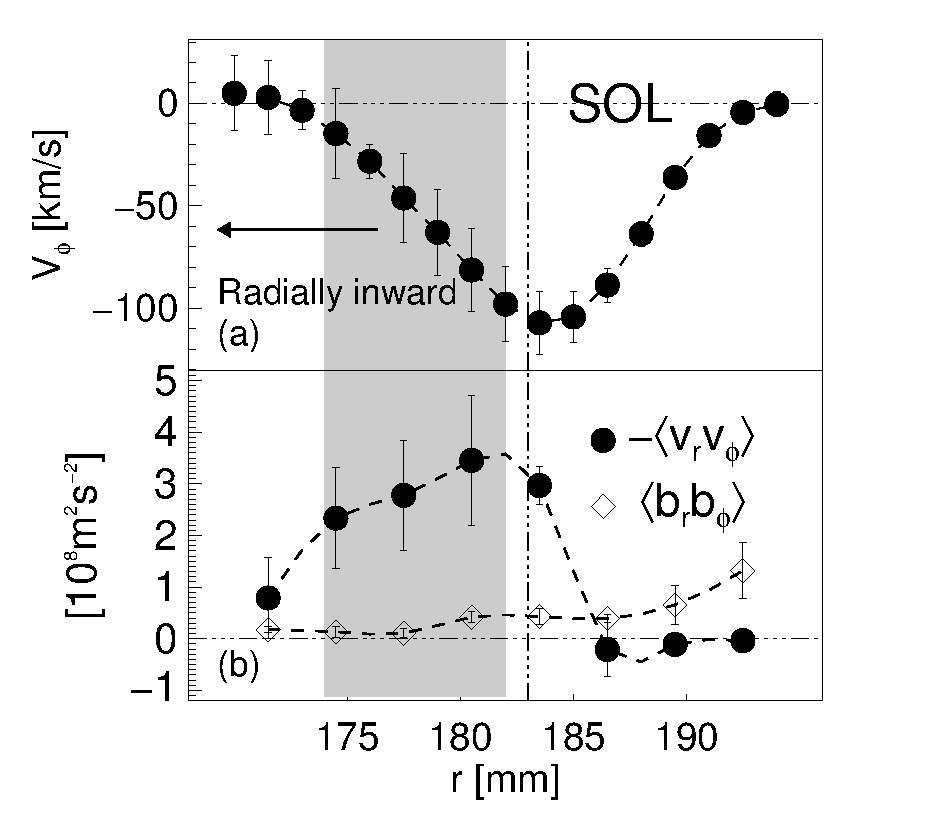
\includegraphics[height=3.4cm]{Profili-Rs-velocity} \\
{\tiny PRL 94 p. 135001, NF 45 p. 761, PPCF 48 p. S193}
\end{center}
\end{column}
}
\onslide<3>{\begin{column}{0.48\textwidth}
{\small\begin{block}{}
(ii) Transport reduction induced by active modification of
  sheared flow
\end{block}}

\vspace{.36cm}

\begin{center}
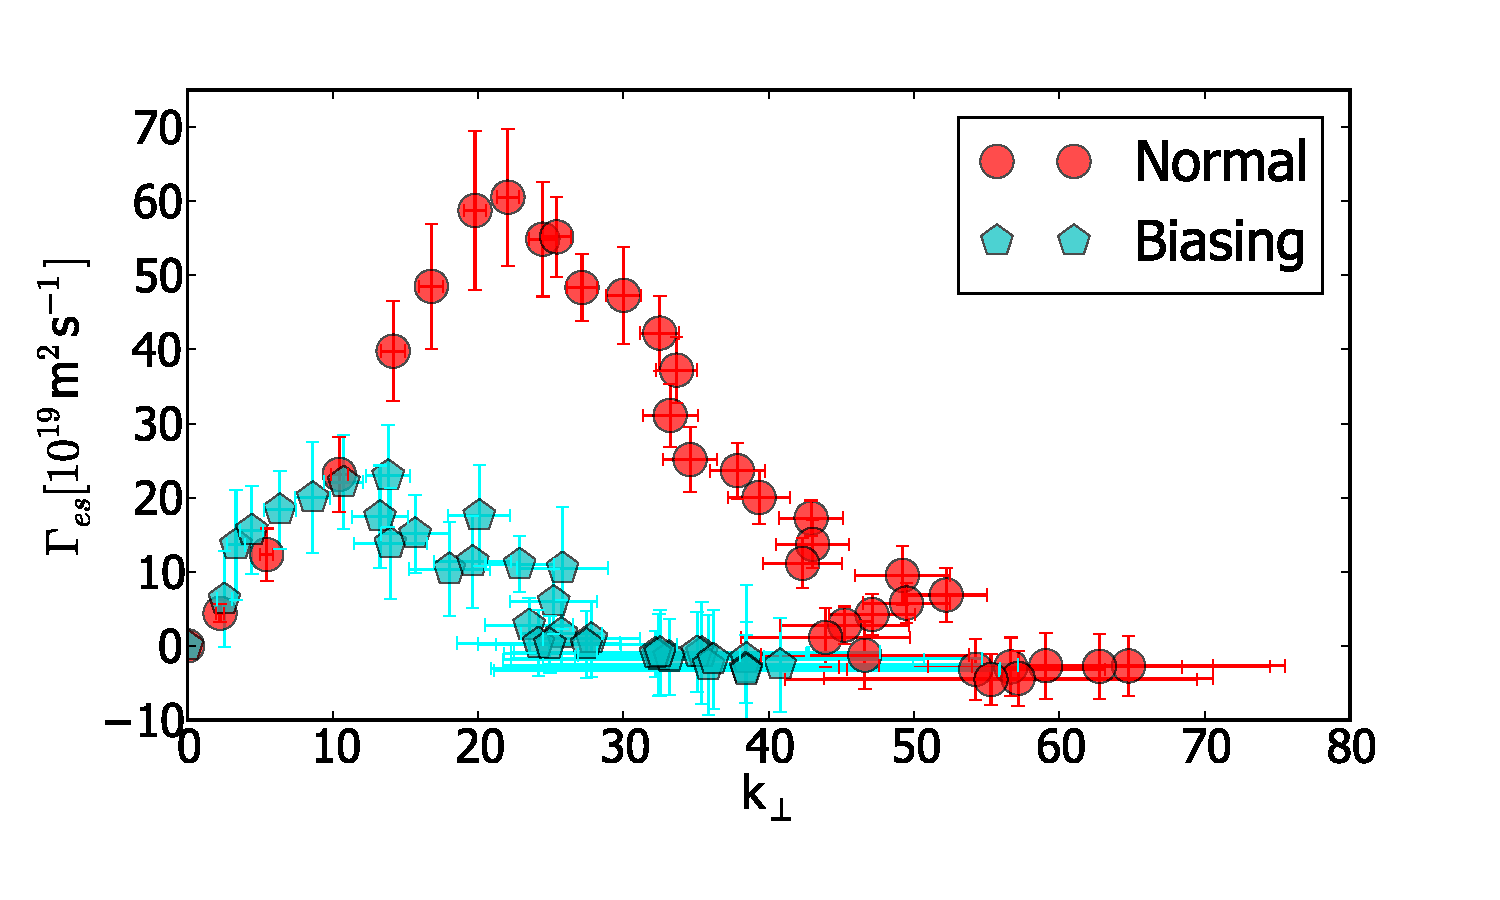
\includegraphics[height=3.4cm]{flux_biasing} \\
{\tiny PPCF 42, p. 83}
\end{center}
\end{column}
}
\end{columns}
\end{itemize}
\end{frame}



\begin{frame}{Coherent structures characterization}
%% per aggiungere la lettera colorata con l'argomento in alto a sx'
\begin{tikzpicture}[remember picture, overlay]
\node [shift={(-0.779 cm,-0.4cm)}]  at (current page.north east)
   {\tikz[baseline=(t1.base)]{\node[fill=ta3chameleon](t1){%
{\Large B}};}
    };
\end{tikzpicture}
%%


\begin{columns}[t]
\begin{column}{0.47\textwidth}
\begin{itemize}
\item Complete characterization of coherent structures responsible for
  intermittency 
\begin{center}
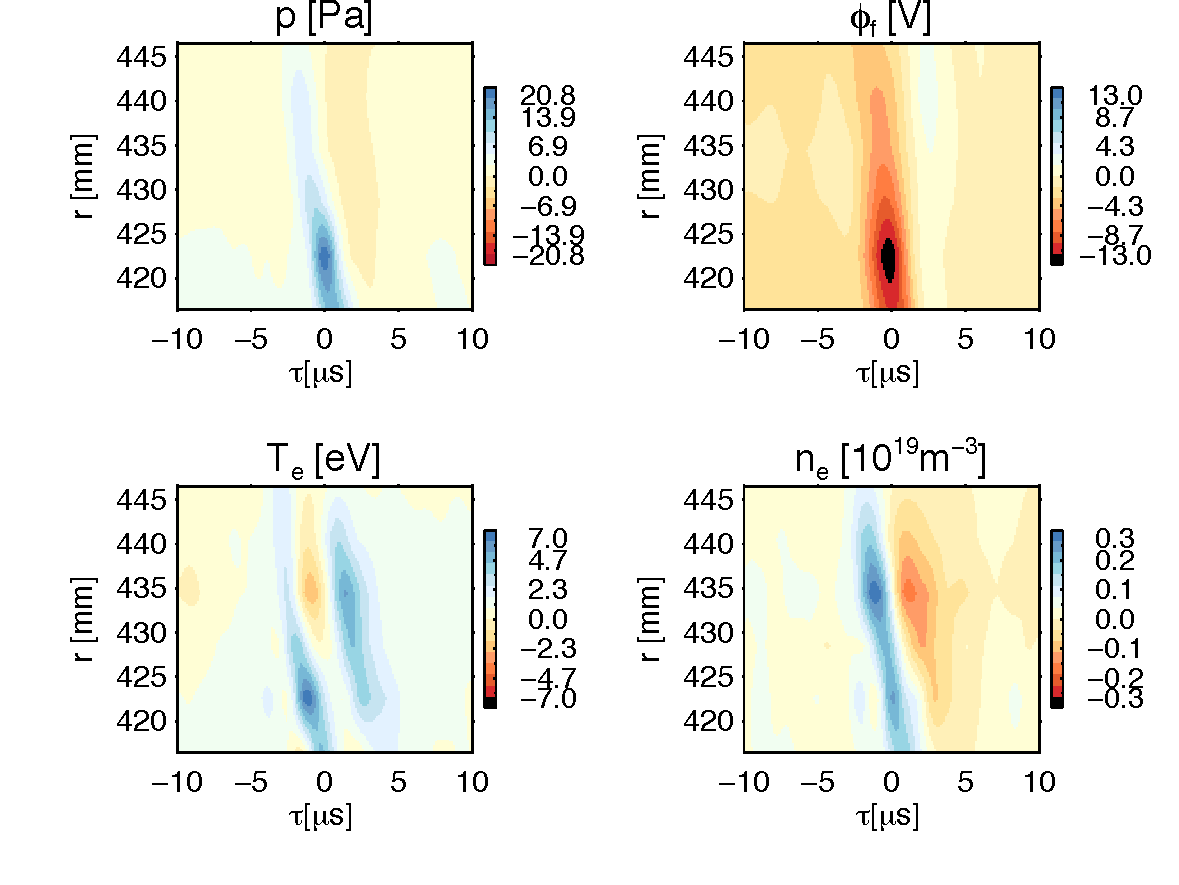
\includegraphics[height=4.5cm]{2Dstructure}
\end{center}
\end{itemize}
\end{column}
\pause
\begin{column}{0.5\textwidth}
\begin{itemize}
\item Evaluation of transport contribution due to coherent structures
\end{itemize}
\begin{center}
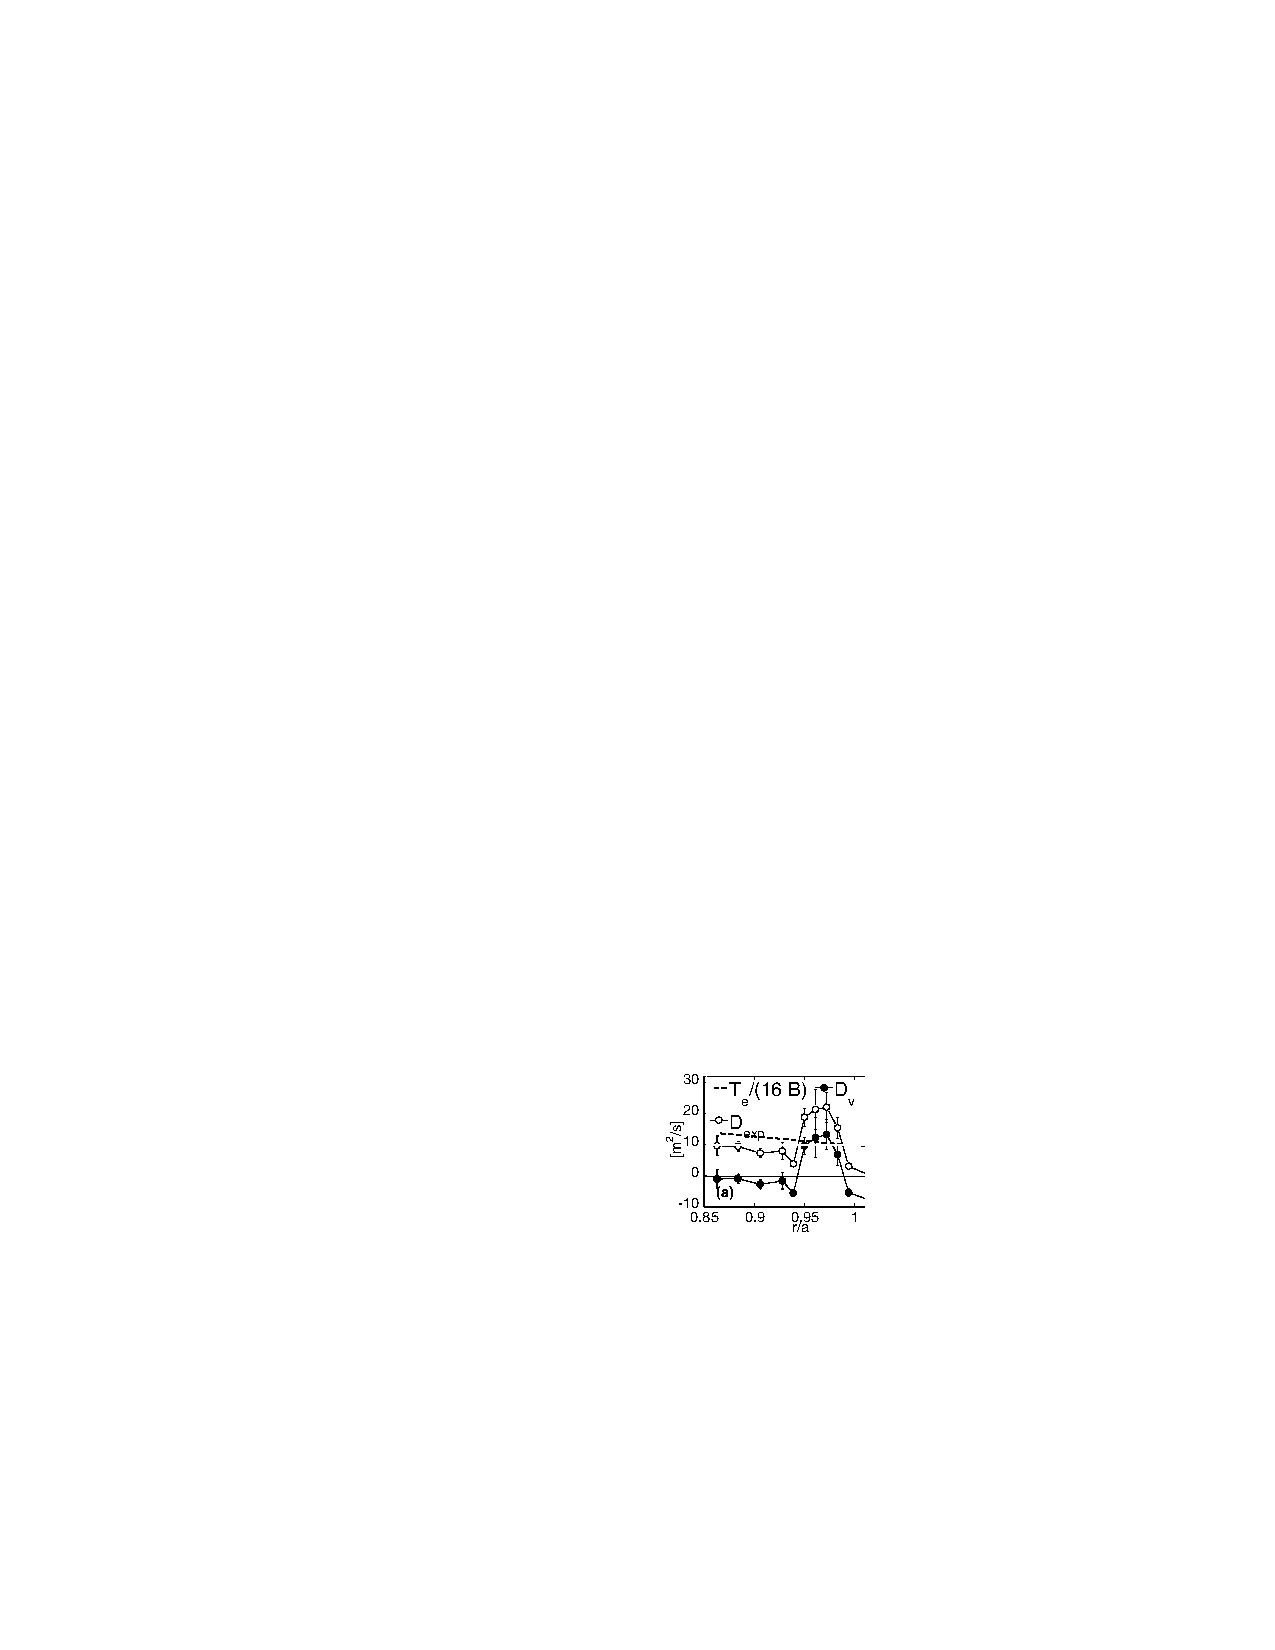
\includegraphics[height=3cm]{structure-diffusivity}
\end{center}
\end{column}
\end{columns}
\begin{center}
{\tiny PRL 93 p.215003, PoP 9 p.4110}
\end{center}
\end{frame}
\begin{frame}{Current filaments}
%% per aggiungere la lettera colorata con l'argomento in alto a sx'
\begin{tikzpicture}[remember picture, overlay]
\node [shift={(-0.779 cm,-0.4cm)}]  at (current page.north east)
   {\tikz[baseline=(t1.base)]{\node[fill=ta3chameleon](t1){%
{\Large B}};}
    };
\end{tikzpicture}
%%
\onslide<1-3>{\begin{itemize}
\item {\small Measurements of parallel plasma current associated to
  \emph{blobs} \& \emph{filaments} in different experiments with
  different magnetic configuration}
\end{itemize}}
\only<1>{
\begin{columns}[c]
\begin{column}{0.6\textwidth}
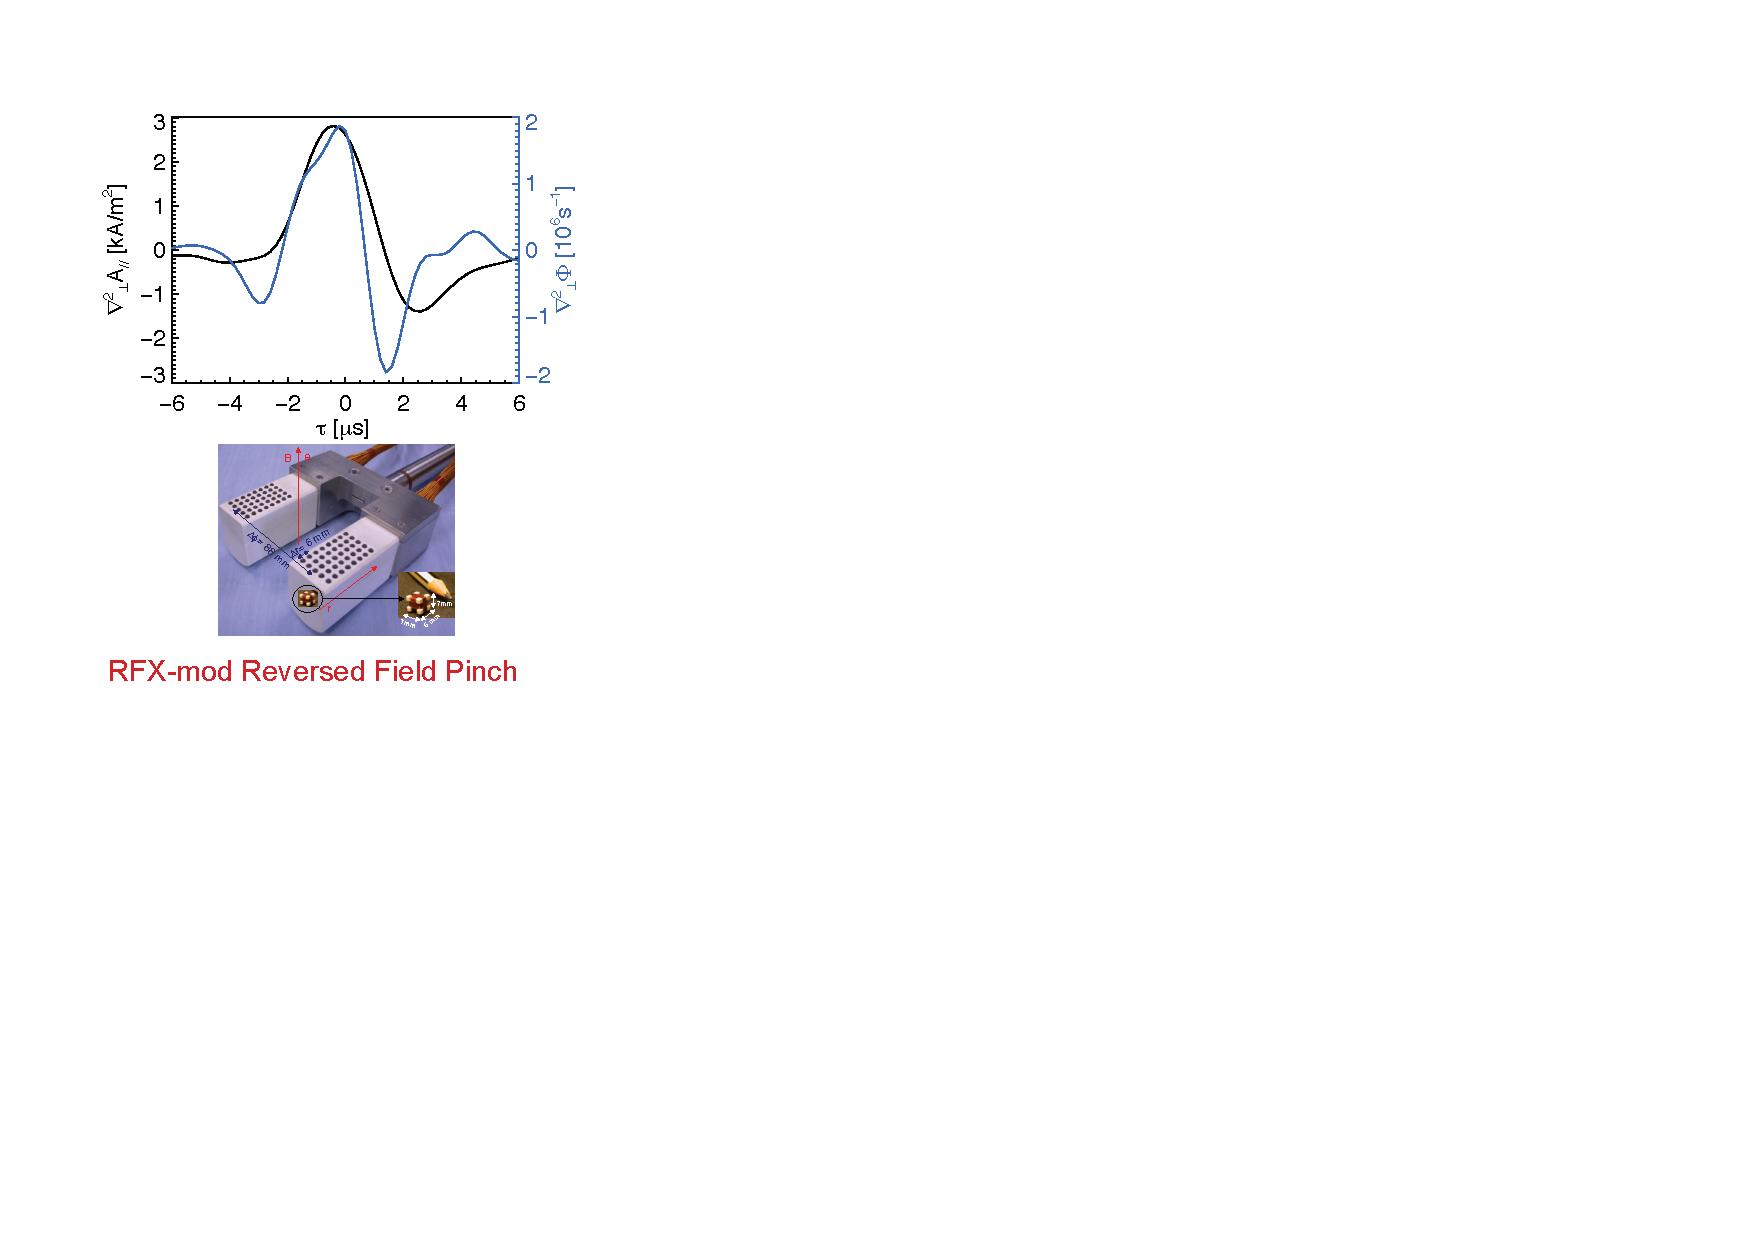
\includegraphics[width=0.78\textwidth]{RFX-current}
\end{column}
\begin{column}{0.4\textwidth}
\begin{block}{}
\begin{itemize}
\item First direct measurements of current filaments associated to plasma
  blob identified as DKA vortex PRL 102 2009, NF 50 2010
\end{itemize}
\end{block}
\end{column}
\end{columns}
}
\only<2>{
\begin{columns}[c]
\begin{column}{0.6\textwidth}
\includegraphics[width=0.58\textwidth]{AUG-current}
\end{column}
\begin{column}{0.4\textwidth}
\begin{block}{}
\begin{itemize}
\item First direct measurements of current asociated to type-I
  filaments (PRL 106, 2011)
\end{itemize}
\end{block}
\end{column}
\end{columns}
}


\only<3>{
\begin{columns}[c]
\begin{column}{0.4\textwidth}
\includegraphics[width=0.78\textwidth]{TORPEX-current}
\end{column}
\begin{column}{0.6\textwidth}
\begin{block}{}
\begin{itemize}
\item First direct 2D map of parallel current associated to an
  interchange-induced plasma blob (PRL 106, 2011)
\end{itemize}
\end{block}
\end{column}
\end{columns}

}


\only<4>{\begin{itemize}
\item Collaboration established to extend studies of current filaments
  to other devices, namely \textcolor{ta3chameleon}{\texttt{TJ-II
      stellarator}}, with a probe which combines vorticity and current
  measurements and \textcolor{ta3skyblue}{\texttt{EAST tokamak}} for
  the studies of ELMs
\begin{center}
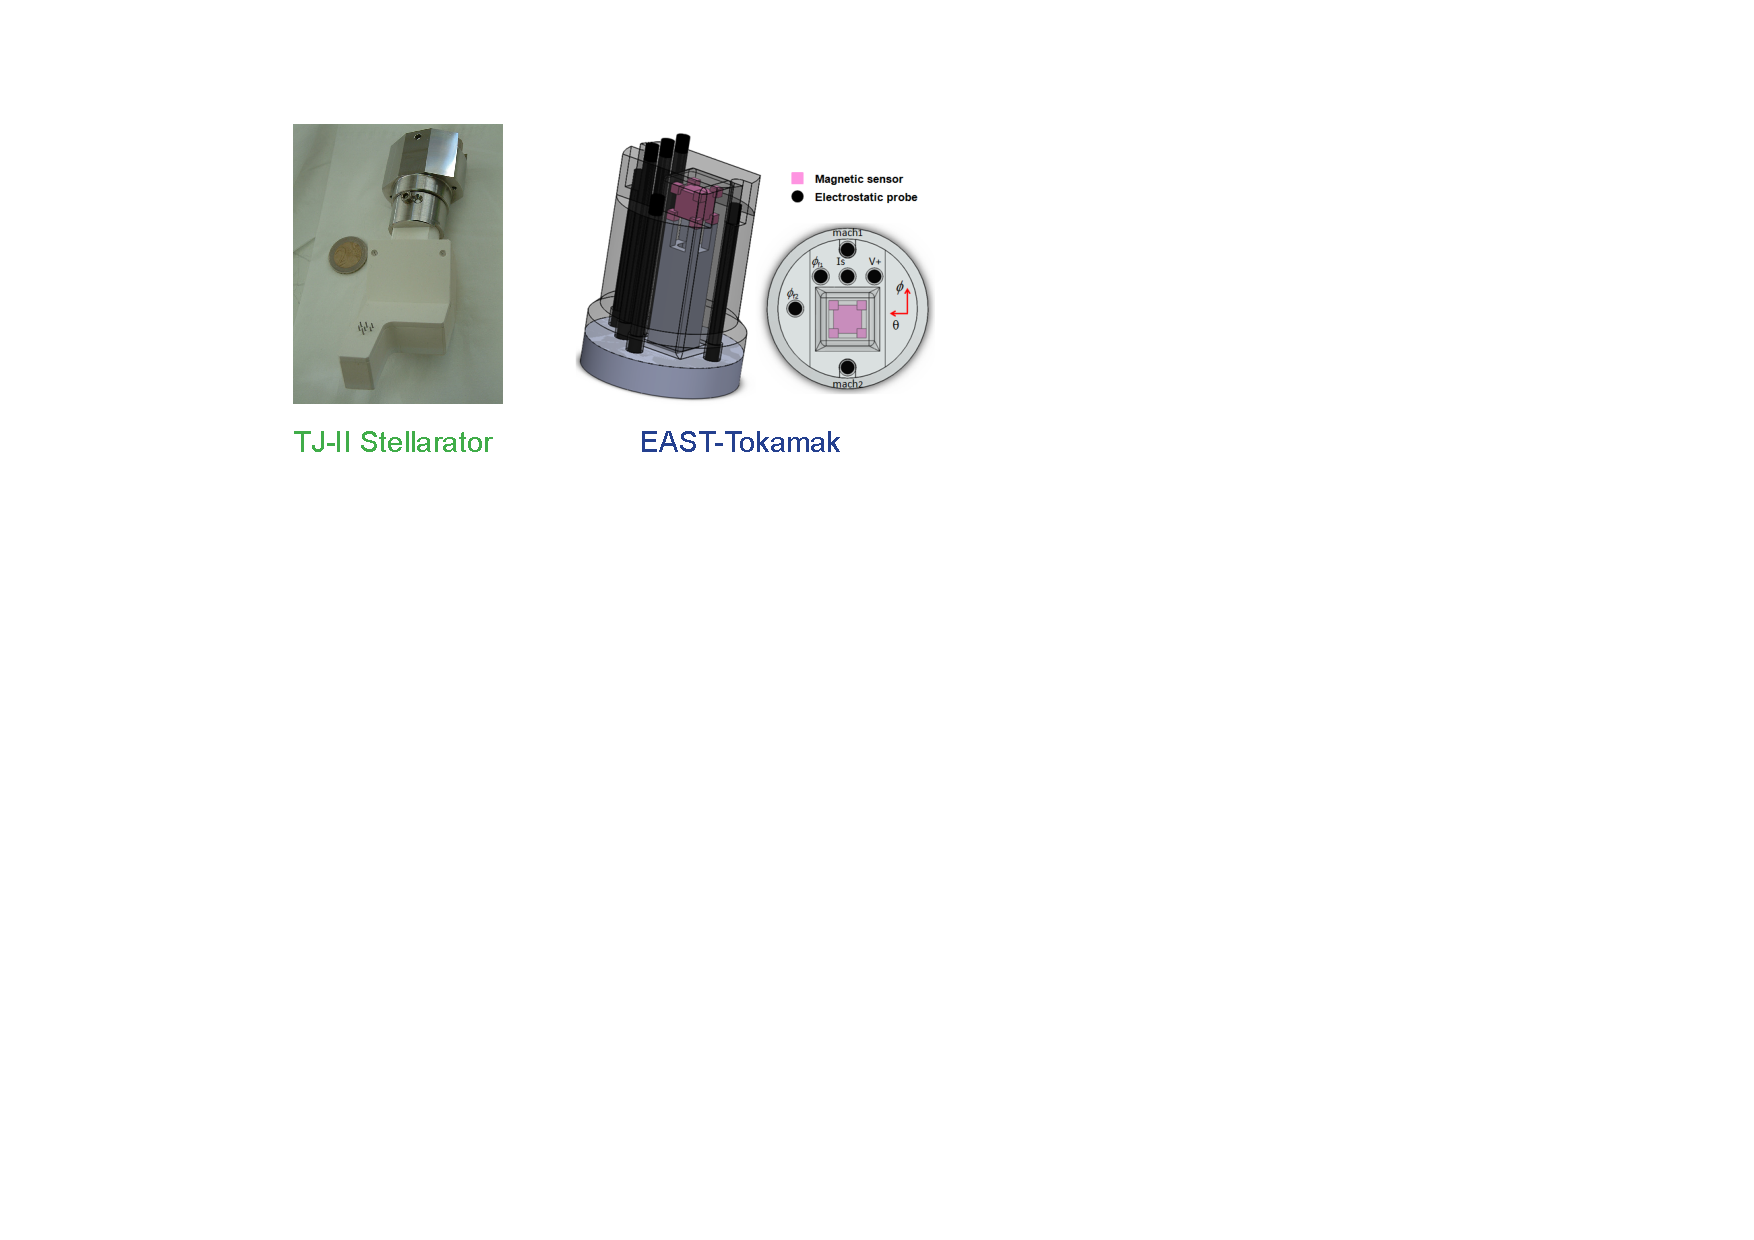
\includegraphics[height=4cm]{collaboration}
\end{center}
\end{itemize}
}\end{frame}


\begin{frame}{Helical plasmas}
%% per aggiungere la lettera colorata con l'argomento in alto a sx'
\begin{tikzpicture}[remember picture, overlay]
\node [shift={(-0.779 cm,-0.4cm)}]  at (current page.north east)
   {\tikz[baseline=(t1.base)]{\node[fill=tascarletred](t1){%
{\Large C}};}
    };
\end{tikzpicture}
%%
\only<1>{\vspace{1cm}

\begin{columns}[c]
\begin{column}{0.4\textwidth}
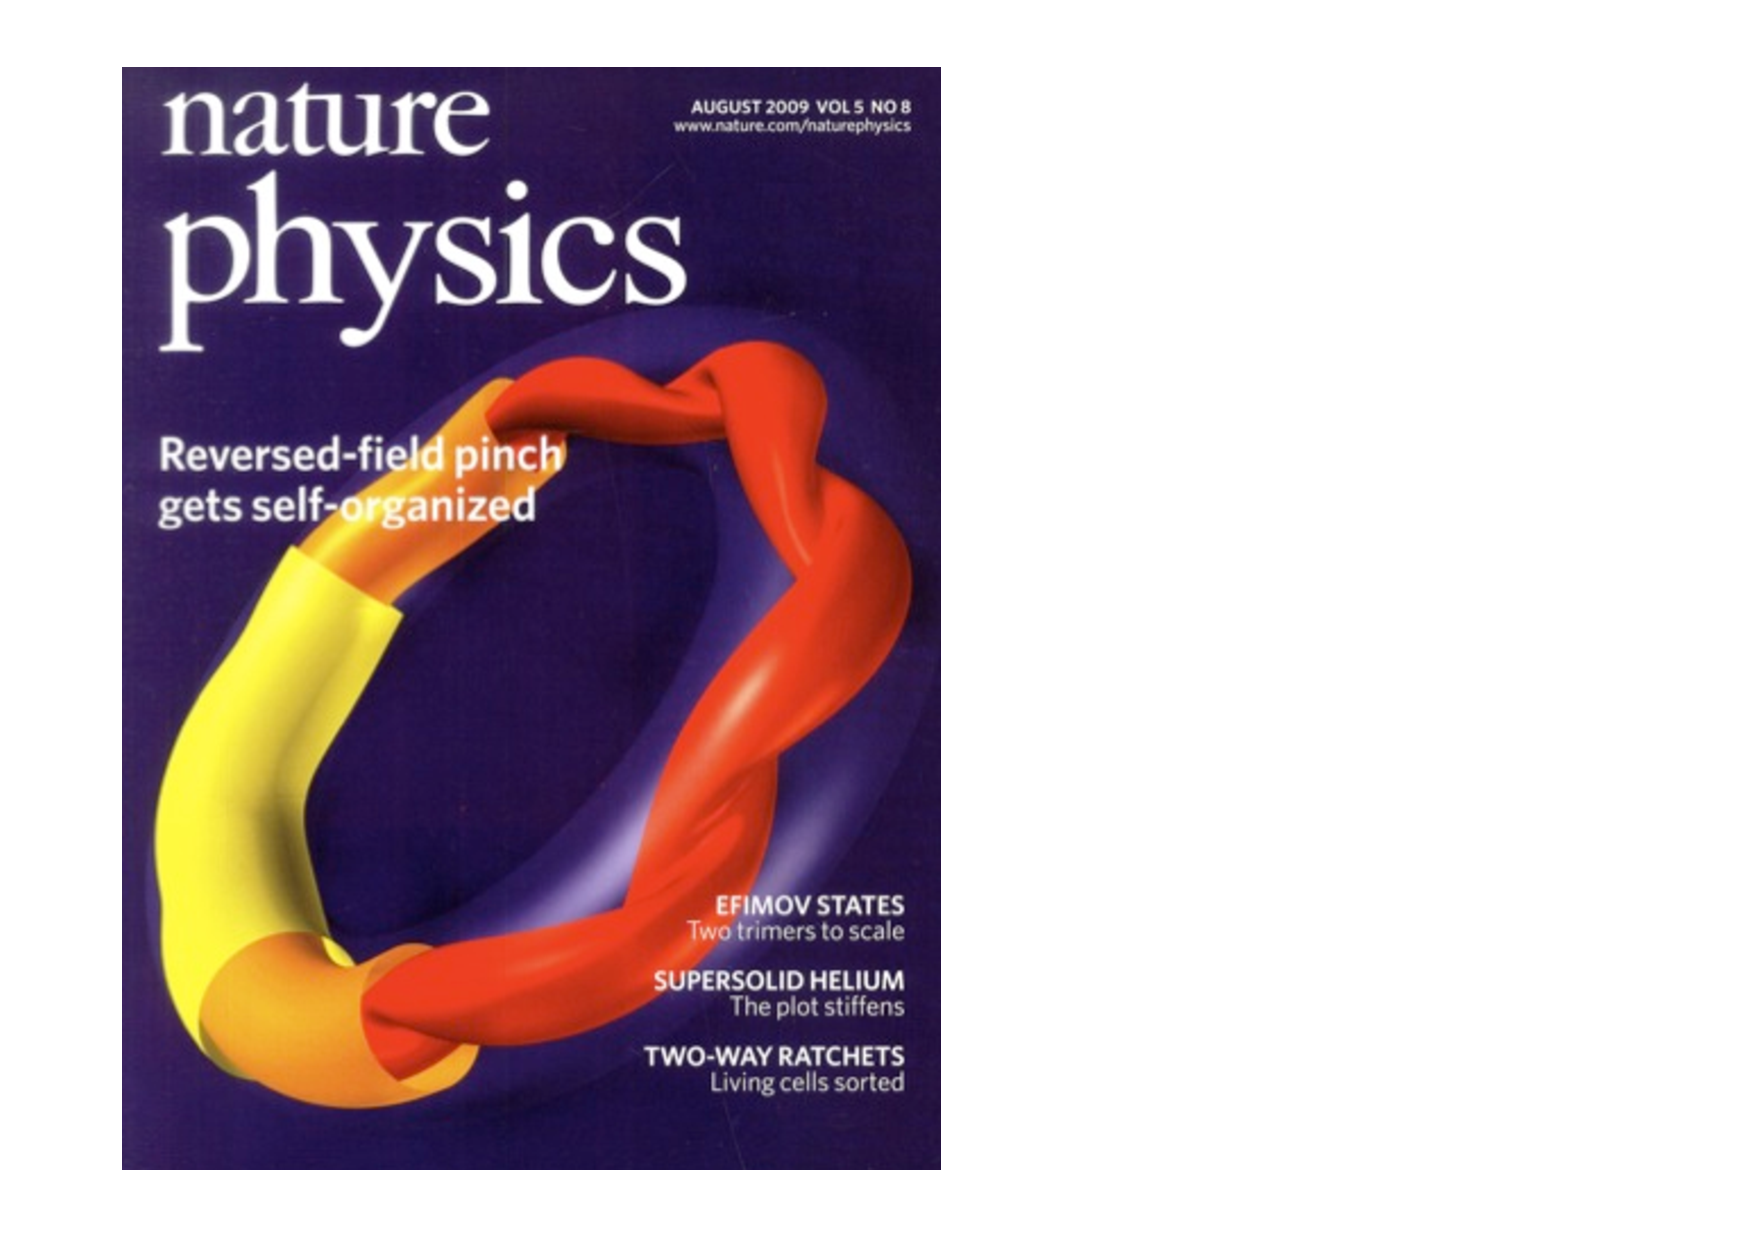
\includegraphics[height=5cm]{copertina}
\end{column}
\begin{column}{0.58\textwidth}
\begin{itemize}
\item {\large Observation and characterization of spontaneous helical plasmas
  developing in high current Reversed Field Pinch operation {\small
    Nat. Phys. 5 pp. 570}}
\end{itemize}
\end{column}
\end{columns}
}

\only<2>{
\begin{columns}[c]
\begin{column}{0.5\textwidth}
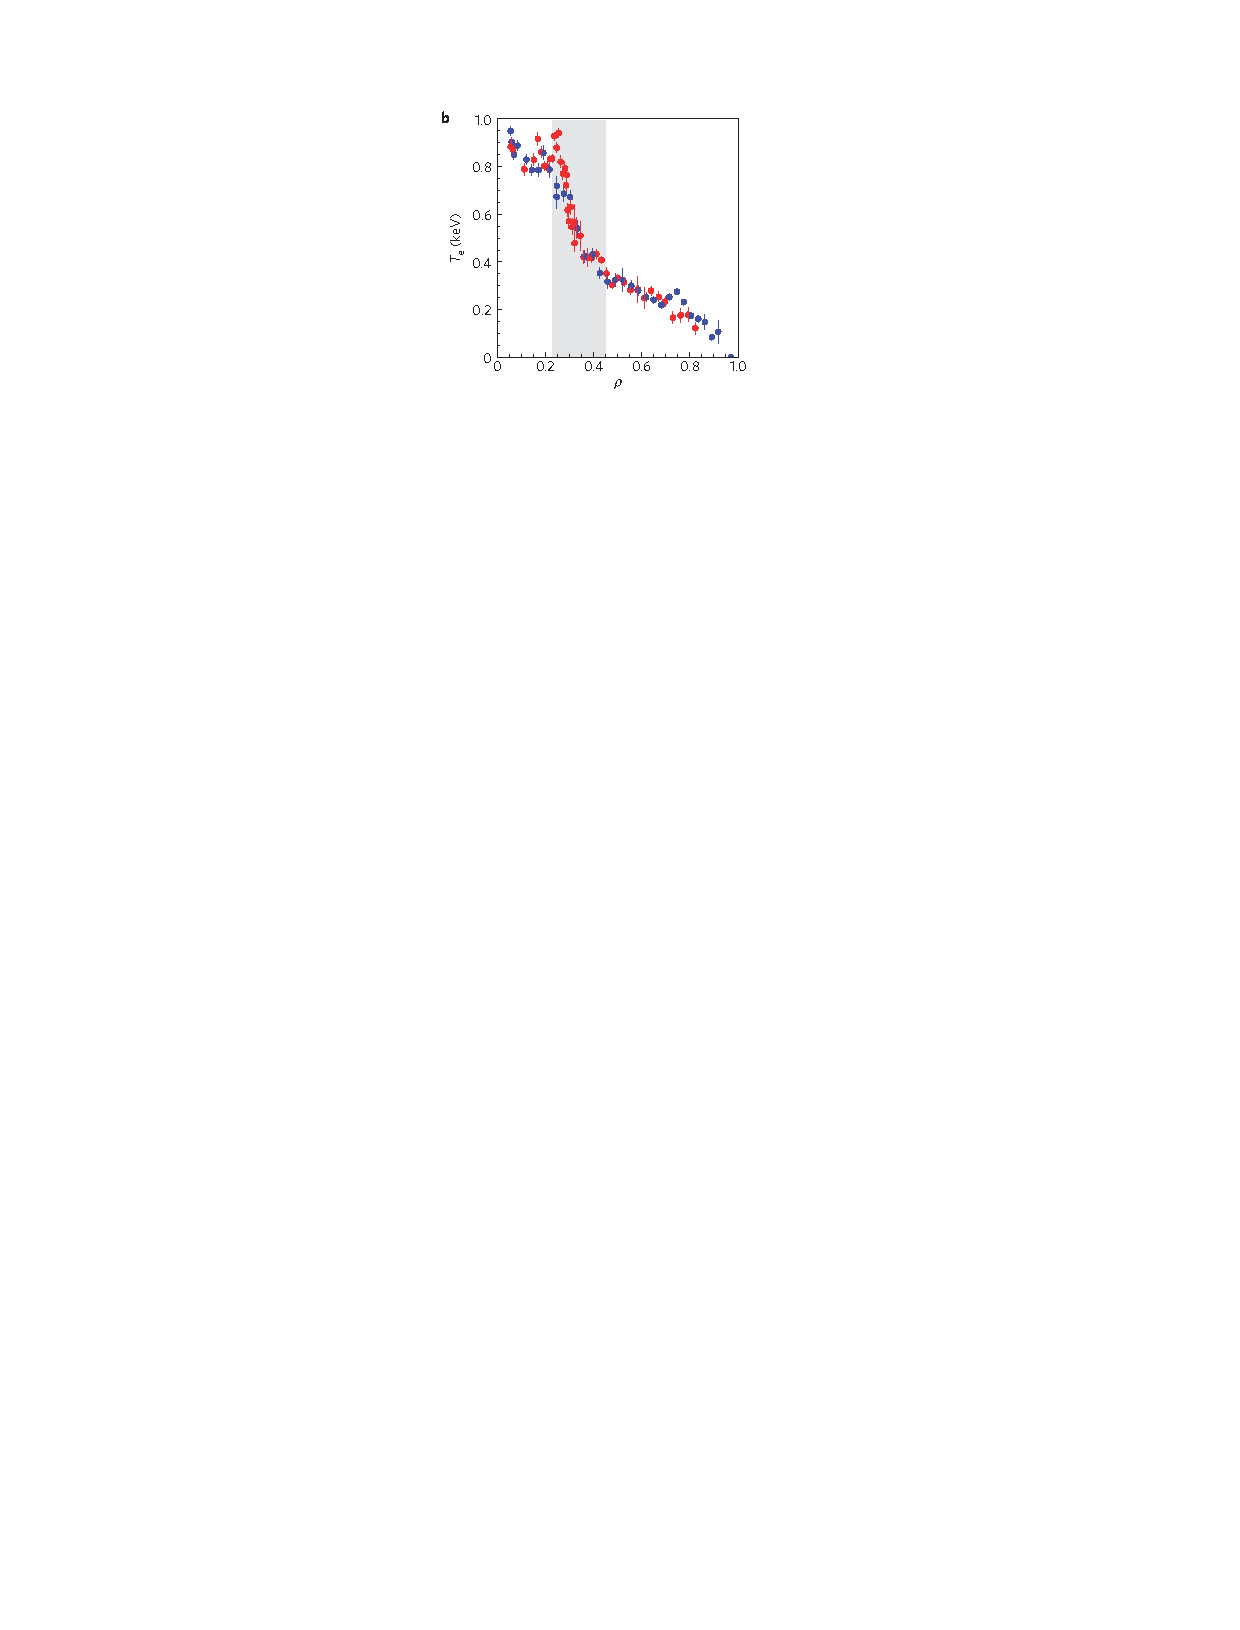
\includegraphics[width=6.cm]{RFX-TraBarr}
\end{column}
\begin{column}{0.5\textwidth}
\begin{block}{}
\begin{itemize}
\item With the appearence of a transport barrier located in the region
  of a local maxima of $q$ value
\end{itemize}
\end{block}
\end{column}
\end{columns}
}



\only<3>{
\begin{columns}[c]
\begin{column}{0.5\textwidth}
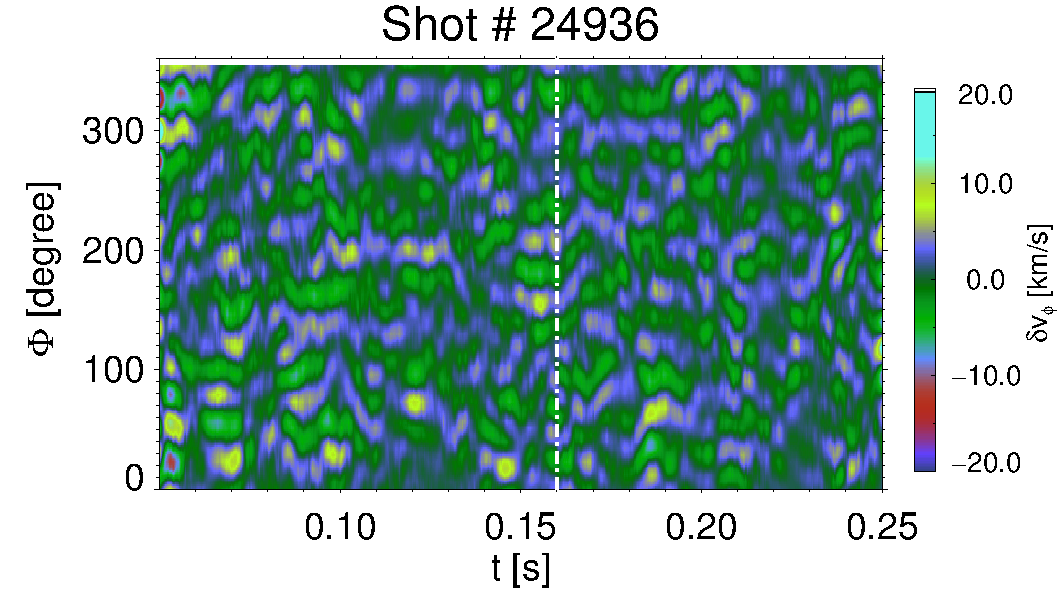
\includegraphics[height=5cm]{helical-flow}
\end{column}
\begin{column}{0.5\textwidth}
\begin{itemize}
\item Ambipolar electric field builds up as a response to the magnetic perturbation
  causing a perpendicular flow with the same periodicity of the helical perturbation
\end{itemize}
\end{column}
\end{columns}
}

\only<4>{
\begin{columns}[c]
\begin{column}{0.5\textwidth}
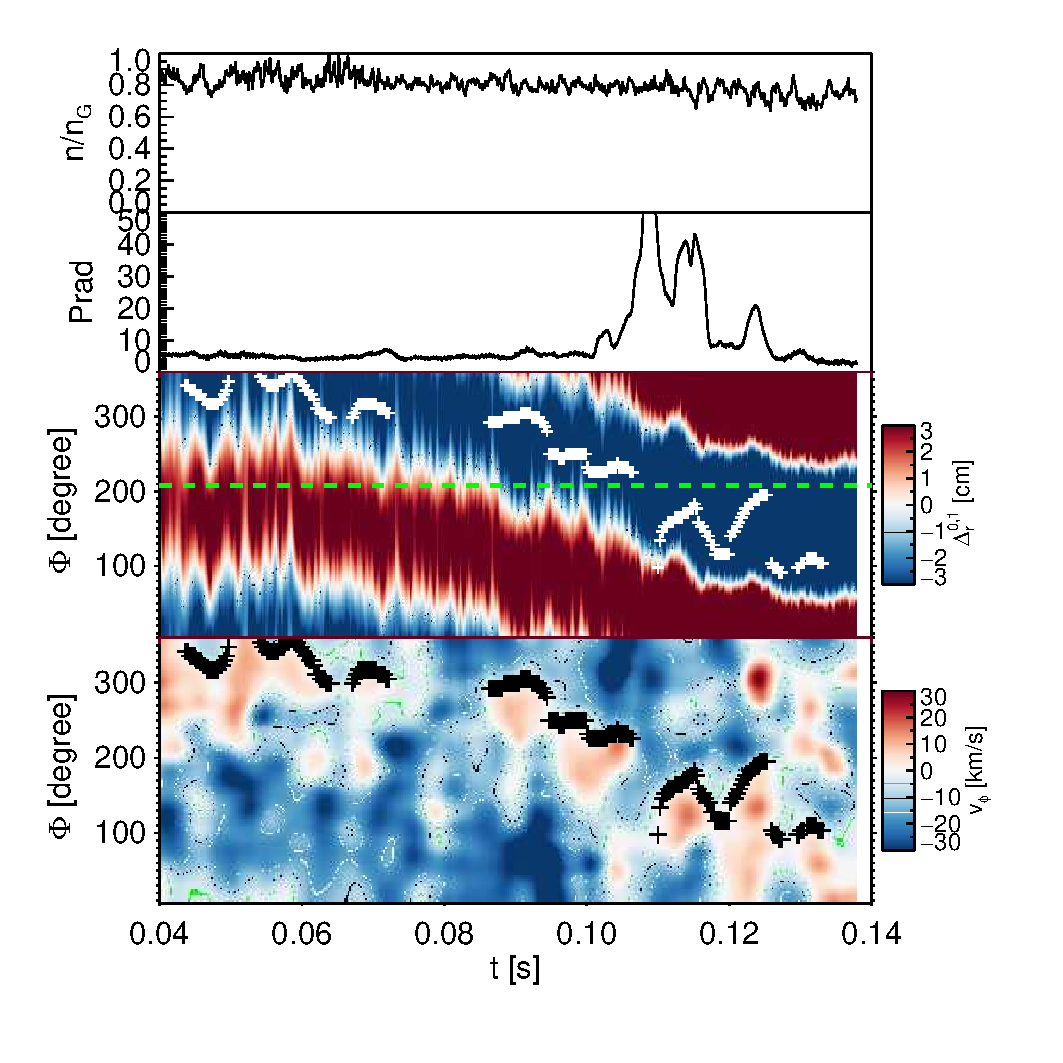
\includegraphics[height=8cm]{Shot26317_ShiftFlow}
\end{column}
\begin{column}{0.5\textwidth}
\begin{itemize}
\item Similar phenomenology appears in High density regime
\item In this case, radiative collapse caused by density accumulation caused by perpendicular flow inversion
\item Accumulation point coincides with the X-point of the magnetic islands (asterisks track accumulation point)
 \end{itemize}
\end{column}
\end{columns}
}


\end{frame}

\begin{frame}{Coordination experience:RFX-mod}
%% per aggiungere la lettera colorata con l'argomento in alto a sx'
% \begin{tikzpicture}[remember picture, overlay]
% \node [shift={(-0.779 cm,-0.3cm)}]  at (current page.north east)
%    {\tikz[baseline=(t1.base)]{\node[fill=ta3skyblue](t1){%
% {\large D}};}
%     };
% \end{tikzpicture}
%%
\begin{itemize}[<+->]
\item RFX-mod scientific program is coordinate by Task Force Leaders which determines
  priorities among experimental proposals in collaborations with
  Scientific Coordinators
\item Scientific objectives are determined on the basis of
  experimental proposals (around 100 experimental proposals for each year)
\item Experimental time appointed on the basis of scientific
  priorities and machine condition in order to optimize the
  experimental time
\item I've been appointed task force leaders for two subsequent years:
  \begin{description}
  \item[2009] TFL for task force \emph{Particle, momentum and energy transport}
  \item[2010] TFL for task force \emph{Physics integration for high
      performance RFP}
  \end{description}
\end{itemize} 
\end{frame}


\begin{frame}{Coordination experience: EFDA Transport topical Group}
  \begin{itemize}[<+->]
\item In 2011 I've been appointed as coordinator of the working group
  \emph{3D field effects in edge and SOL and diagnostic development}
  for the Transport-topical group
\item Monitoring and coordination of activities on the topics
  highlighted coming from 11 different European Associations
\item Discussion stimulated through remote meeting and shared wiki
  page information
\item Monitor of the activities exposed to the STAC committee 
 
\end{itemize} 
\end{frame}




\end{document}
